\documentclass[journal, a4paper]{IEEEtran}

% some very useful LaTeX packages include:

\usepackage{amsfonts,amssymb}
%\usepackage{cite}      % Written by Donald Arseneau
                        % V1.6 and later of IEEEtran pre-defines the format
                        % of the cite.sty package \cite{} output to follow
                        % that of IEEE. Loading the cite package will
                        % result in citation numbers being automatically
                        % sorted and properly "ranged". i.e.,
                        % [1], [9], [2], [7], [5], [6]
                        % (without using cite.sty)
                        % will become:
                        % [1], [2], [5]--[7], [9] (using cite.sty)
                        % cite.sty's \cite will automatically add leading
                        % space, if needed. Use cite.sty's noadjust option
                        % (cite.sty V3.8 and later) if you want to turn this
                        % off. cite.sty is already installed on most LaTeX
                        % systems. The latest version can be obtained at:
                        % http://www.ctan.org/tex-archive/macros/latex/contrib/supported/cite/

\usepackage{graphicx}   % Written by David Carlisle and Sebastian Rahtz
                        % Required if you want graphics, photos, etc.
                        % graphicx.sty is already installed on most LaTeX
                        % systems. The latest version and documentation can
                        % be obtained at:
                        % http://www.ctan.org/tex-archive/macros/latex/required/graphics/
                        % Another good source of documentation is "Using
                        % Imported Graphics in LaTeX2e" by Keith Reckdahl
                        % which can be found as esplatex.ps and epslatex.pdf
                        % at: http://www.ctan.org/tex-archive/info/

%\usepackage{psfrag}    % Written by Craig Barratt, Michael C. Grant,
                        % and David Carlisle
                        % This package allows you to substitute LaTeX
                        % commands for text in imported EPS graphic files.
                        % In this way, LaTeX symbols can be placed into
                        % graphics that have been generated by other
                        % applications. You must use latex->dvips->ps2pdf
                        % workflow (not direct pdf output from pdflatex) if
                        % you wish to use this capability because it works
                        % via some PostScript tricks. Alternatively, the
                        % graphics could be processed as separate files via
                        % psfrag and dvips, then converted to PDF for
                        % inclusion in the main file which uses pdflatex.
                        % Docs are in "The PSfrag System" by Michael C. Grant
                        % and David Carlisle. There is also some information
                        % about using psfrag in "Using Imported Graphics in
                        % LaTeX2e" by Keith Reckdahl which documents the
                        % graphicx package (see above). The psfrag package
                        % and documentation can be obtained at:
                        % http://www.ctan.org/tex-archive/macros/latex/contrib/supported/psfrag/

%\usepackage{subfigure} % Written by Steven Douglas Cochran
                        % This package makes it easy to put subfigures
                        % in your figures. i.e., "figure 1a and 1b"
                        % Docs are in "Using Imported Graphics in LaTeX2e"
                        % by Keith Reckdahl which also documents the graphicx
                        % package (see above). subfigure.sty is already
                        % installed on most LaTeX systems. The latest version
                        % and documentation can be obtained at:
                        % http://www.ctan.org/tex-archive/macros/latex/contrib/supported/subfigure/

\usepackage{url}        % Written by Donald Arseneau
                        % Provides better support for handling and breaking
                        % URLs. url.sty is already installed on most LaTeX
                        % systems. The latest version can be obtained at:
                        % http://www.ctan.org/tex-archive/macros/latex/contrib/other/misc/
                        % Read the url.sty source comments for usage information.

%\usepackage{stfloats}  % Written by Sigitas Tolusis
                        % Gives LaTeX2e the ability to do double column
                        % floats at the bottom of the page as well as the top.
                        % (e.g., "\begin{figure*}[!b]" is not normally
                        % possible in LaTeX2e). This is an invasive package
                        % which rewrites many portions of the LaTeX2e output
                        % routines. It may not work with other packages that
                        % modify the LaTeX2e output routine and/or with other
                        % versions of LaTeX. The latest version and
                        % documentation can be obtained at:
                        % http://www.ctan.org/tex-archive/macros/latex/contrib/supported/sttools/
                        % Documentation is contained in the stfloats.sty
                        % comments as well as in the presfull.pdf file.
                        % Do not use the stfloats baselinefloat ability as
                        % IEEE does not allow \baselineskip to stretch.
                        % Authors submitting work to the IEEE should note
                        % that IEEE rarely uses double column equations and
                        % that authors should try to avoid such use.
                        % Do not be tempted to use the cuted.sty or
                        % midfloat.sty package (by the same author) as IEEE
                        % does not format its papers in such ways.

\usepackage{amsmath}    % From the American Mathematical Society
                        % A popular package that provides many helpful commands
                        % for dealing with mathematics. Note that the AMSmath
                        % package sets \interdisplaylinepenalty to 10000 thus
                        % preventing page breaks from occurring within multiline
                        % equations. Use:
%\interdisplaylinepenalty=2500
                        % after loading amsmath to restore such page breaks
                        % as IEEEtran.cls normally does. amsmath.sty is already
                        % installed on most LaTeX systems. The latest version
                        % and documentation can be obtained at:
                        % http://www.ctan.org/tex-archive/macros/latex/required/amslatex/math/



% Other popular packages for formatting tables and equations include:

%\usepackage{array}
% Frank Mittelbach's and David Carlisle's array.sty which improves the
% LaTeX2e array and tabular environments to provide better appearances and
% additional user controls. array.sty is already installed on most systems.
% The latest version and documentation can be obtained at:
% http://www.ctan.org/tex-archive/macros/latex/required/tools/

% V1.6 of IEEEtran contains the IEEEeqnarray family of commands that can
% be used to generate multiline equations as well as matrices, tables, etc.

% Also of notable interest:
% Scott Pakin's eqparbox package for creating (automatically sized) equal
% width boxes. Available:
% http://www.ctan.org/tex-archive/macros/latex/contrib/supported/eqparbox/

% *** Do not adjust lengths that control margins, column widths, etc. ***
% *** Do not use packages that alter fonts (such as pslatex).         ***
% There should be no need to do such things with IEEEtran.cls V1.6 and later.


% Your document starts here!
\begin{document}
\begin{titlepage}

\newcommand{\HRule}{\rule{\linewidth}{0.5mm}} % Defines a new command for the horizontal lines, change thickness here

\center % Center everything on the page
 %----------------------------------------------------------------------------------------
%	LOGO SECTION
%----------------------------------------------------------------------------------------

~\\[1cm]

\includegraphics{SCUT.png}\\[2cm] % Include a department/university logo - this will require the graphicx package

%----------------------------------------------------------------------------------------
%	TITLE SECTION
%----------------------------------------------------------------------------------------

\HRule \\[1cm]
{ \huge \bfseries The Experiment Report of \textit{Machine Learning} }\\[0.6cm] % Title of your document
\HRule \\[2cm]
%----------------------------------------------------------------------------------------
%	HEADING SECTIONS
%----------------------------------------------------------------------------------------


\textsc{\LARGE \textbf{School:} School of Software Engineering}\\[1cm]
\textsc{\LARGE \textbf{Subject:} Software Engineering}\\[2cm]


%----------------------------------------------------------------------------------------
%	AUTHOR SECTION
%----------------------------------------------------------------------------------------

\begin{minipage}{0.4\textwidth}
\begin{flushleft} \large
\emph{Author:}\\
Haipeng Deng % Your name
\end{flushleft}
\end{minipage}
~
\begin{minipage}{0.4\textwidth}
\begin{flushright} \large
\emph{Supervisor:} \\
Mingkui Tan% Supervisor's Name
\end{flushright}
\end{minipage}\\[2cm]
~
\begin{minipage}{0.4\textwidth}
\begin{flushleft} \large
\emph{Student ID:}\\
201730686193
\end{flushleft}
\end{minipage}
~
\begin{minipage}{0.4\textwidth}
\begin{flushright} \large
\emph{Grade:} \\
Undergraduate
\end{flushright}
\end{minipage}\\[2cm]

% If you don't want a supervisor, uncomment the two lines below and remove the section above
%\Large \emph{Author:}\\
%John \textsc{Smith}\\[3cm] % Your name

%----------------------------------------------------------------------------------------
%	DATE SECTION
%----------------------------------------------------------------------------------------

{\large \today}\\[2cm] % Date, change the \today to a set date if you want to be precise


%----------------------------------------------------------------------------------------

\vfill % Fill the rest of the page with whitespace

\end{titlepage}

% Define document title and author
	\title{Recommender System Based on Matrix Decomposition}
	\maketitle

% Write abstract here
\begin{abstract}
This report introduces my work in lab5, where I built a recommending system based on matrix factorization and optimized it using the strategy of stochastic gradient descent.
\end{abstract}

% Each section begins with a \section{title} command
\section{Introduction}
	% \PARstart{}{} creates a tall first letter for this first paragraph
\PARstart{T}{he} recommender system has been developed as an independent discipline for nearly twenty years but not yet has a precise definition. Several strategies have been proposed in the way to constructing a more accurate and more useful model, such as Content-based Algorithm, Item-based Collaborative Filtering Algorithm and Matrix Factorization Algorithm. In this lab, we will work on a Matrix Factorization model, which put the observed samples in a sparse matrix and try to decompose it through introducing a new parameter K, which tries to identify the potential features of each user and each item. The main goals of the lab are completely generating a movie recommender system and cultivate engineering ability under a small dataset.

% Main Part
\section{Methods and Theory}
Before constructing a recommender system using matrix factorization, there are some concepts we need to introduce. A matrix $R \in \mathbb{R} ^ {m*n}$ is a sparse rating matrix for m users and n items(movies in this case). An observed samples $r_{u,i}$ (means the rate of user $u$ towards item(movie) $i$) will be represented as a specific value in $R$. In the matrix factorization method we use, we will try to decompose $R$ into two matrices $P \in \mathbb{R} ^ {m*k}$ and $Q \in \mathbb{R} ^ {k*n}$ where k denotes potential features for each user and movie.
\begin{figure}[!hbt]
	% Center the figure.
	\begin{center}
	% Include the eps file, scale it such that it's width equals the column width. You can also put width=8cm for example...
	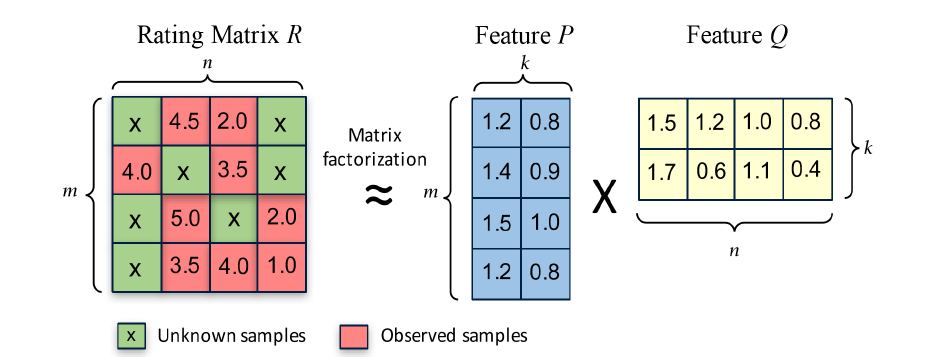
\includegraphics[width=\columnwidth]{matrix_decompose.png}
	% Create a subtitle for the figure.
	\caption{An illustration of matrix factorization (m=4, n=4, k=2).}
	% Define the label of the figure. It's good to use 'fig:title', so you know that the label belongs to a figure.
	\label{fig1}
	\end{center}
\end{figure}\\
After confirming the basic skeleton of our model, the next step is to determine how we evaluate the goodness of it and the way we optimize it. A naive loss function is squared error loss:
\begin{equation}
    L(r_{u,i},\hat{r}_{u,i}) = (r_{u,i}-\hat{r}_{u,i})^2
\end{equation}\\
Besides, there are two ways to minimize the loss on our lab guidance alternate least squares optimization(ALS) and stochastic gradient descent method(SGD). I chose SGD as my strategy to optimize, because it is a simple and scalable to large-scale datasets way compared to ALS.\\
In stochastic gradient descent, we define the loss function as below:
\begin{equation}
    L = \sum_{u,i\in \Omega} (r_{u,i} - p_u^T q_i)^2 + \lambda_p||p_u||^2+\lambda_q||q_i||^2
\end{equation}\\
$r_{u,i}$ denotes the actual rating of user u for item i.
$\Omega$ denotes the set of observed samples from rating matrix R.
$\lambda_p$ and $\lambda_q$ are regularization parameters to avoid overtting.
In order to minimize the loss and update our matrices P and Q, we randomly pick an observed sample $r_{u,i}$ in the sparse matrix R and there are two other important formulas which we use to calculate gradients:
\begin{align}
    \frac{\partial l}{\partial p_u} = E_{u,i}(-q_i)+\lambda_pp_u & \\
    \frac{\partial l}{\partial q_i} = E_{u,i}(-p_u)+\lambda_qq_i
\end{align}\\
In the equations above, $p_u$ denotes the uth user's column vector while $q_i$ denotes the ith movie's column vector. They both have shape k * 1\\
The following step is to update the feature matrices P and Q with learning rate $\alpha$ making use of the gradients we computed:
\begin{align}
    p_u = p_u + \alpha\frac{\partial l}{\partial p_u} & \\
    q_i = q_i + \alpha\frac{\partial l}{\partial q_i}
\end{align}\\
We will repeat the steps above until the loss converge.

\section{Experiments}
\subsection{Dataset}
In this lab we Utilize the 'MovieLens-100k dataset' which Consists 10,000 comments from 943 users out of 1682 movies. At least, each user comment 20 videos. Users and movies are numbered consecutively from number 1 respectively. The data is sorted randomly.

\subsection{Implementation}
Firstly, I decided to use u1.base as my train data and u1.test as my test data, then I read the data set to generate my matrix R and fill 0 for null values. According to the principle that $k << min(m,n)$, I finally chose $k = 50, \lambda_p = 0.5, \lambda_q = 0.5 \alpha = 0.01$ as my input hyperparameters. To perform stochastic gradient descent, I randomly selected an observed sample $r_{u,i}$ from observed set, then calculated the gradient $\frac{\partial l}{\partial p_u} \quad, \frac{\partial l}{\partial q_i}$ to the loss function. Next, I updated the feature matrices P and Q with learning rate $alpha$ and gradient using formula (5) (6). I repeated the above processes until convergence.
\begin{figure}[!hbt]
	% Center the figure.
	\begin{center}
	% Include the eps file, scale it such that it's width equals the column width. You can also put width=8cm for example...
	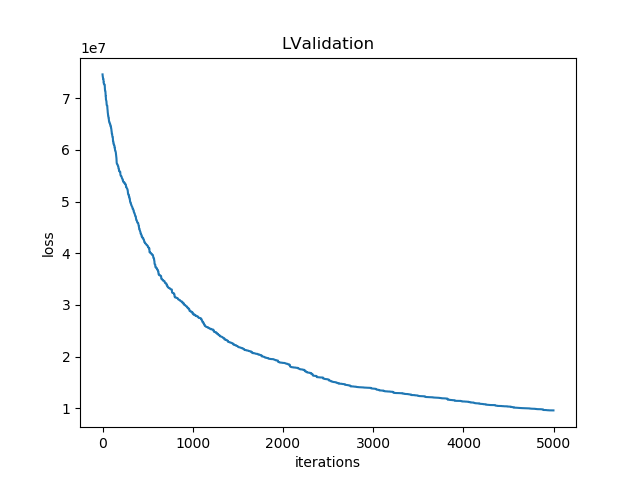
\includegraphics[width=\columnwidth]{result.png}
	% Create a subtitle for the figure.
	\caption{The change of Lvalidation.}
	% Define the label of the figure. It's good to use 'fig:title', so you know that the label belongs to a figure.
	\label{fig2}
	\end{center}
\end{figure}
\par


\section{Conclusion}
	To summarize, I feel this lab very inspiring and beneficial for me. Instead of reading and deriving the theory and formulas in books and slices, it offers us a practical way to practise machine learning.


% Your document ends here!
\end{document}
